% bei Standalone in documentclass noch:
% \RequirePackage{luatex85}

\documentclass[captions=tableheading, titlepage= firstiscover, parskip = half , bibliography=totoc]{scrartcl}
%paper = a5 für andere optinen
% titlepage= firstiscover
% bibliography=totoc für bibdateien
% parskip=half  Veränderung um Absätze zu verbessern

\usepackage{scrhack} % nach \documentclass
\usepackage[aux]{rerunfilecheck}
\usepackage{polyglossia}
\usepackage[style=numeric, backend=biber]{biblatex} % mit [style = alphabetic oder numeric] nach polyglossia
\addbibresource{lit.bib}
\setmainlanguage{german}

\usepackage[autostyle]{csquotes}
\usepackage{amsmath} % unverzichtbare Mathe-Befehle
\usepackage{amssymb} % viele Mathe-Symbole
\usepackage{mathtools} % Erweiterungen für amsmath
\usepackage{fontspec} % nach amssymb
% muss ins document: \usefonttheme{professionalfonts} % für Beamer Präsentationen
\usepackage{longtable}

\usepackage[
math-style=ISO,    % \
bold-style=ISO,    % |
sans-style=italic, % | ISO-Standard folgen
nabla=upright,     % |
partial=upright,   % /
]{unicode-math} % "Does exactly what it says on the tin."
\setmathfont{Latin Modern Math}
% \setmathfont{Tex Gyre Pagella Math} % alternativ

\usepackage[
% die folgenden 3 nur einschalten bei documenten
locale=DE,
separate-uncertainty=true, % Immer Fehler mit ±
per-mode=symbol-or-fraction, % m/s im Text, sonst \frac
]{siunitx}

% alternativ:
% per-mode=reciprocal, % m s^{-1}
% output-decimal-marker=., % . statt , für Dezimalzahlen

\usepackage[
version=4,
math-greek=default,
text-greek=default,
]{mhchem}

\usepackage[section, below]{placeins}
\usepackage{caption} % Captions schöner machen
\usepackage{graphicx}
\usepackage{grffile}
\usepackage{subcaption}

% \usepackage{showframe} Wenn man die Ramen sehen will

\usepackage{float}
\floatplacement{figure}{htbp}
\floatplacement{table}{htbp}

\usepackage{mhchem} %chemische Symbole Beispiel: \ce{^{227}_{90}Th+}


\usepackage{booktabs}

 \usepackage{microtype}
 \usepackage{xfrac}

 \usepackage{expl3}
 \usepackage{xparse}

 % \ExplSyntaxOn
 % \NewDocumentComman \I {}  %Befehl\I definieren, keine Argumente
 % {
 %    \symup{i}              %Ergebnis von \I
 % }
 % \ExplSyntaxOff

 \usepackage{pdflscape}
 \usepackage{mleftright}

 % Mit dem mathtools-Befehl \DeclarePairedDelimiter können Befehle erzeugen werden,
 % die Symbole um Ausdrücke setzen.
 % \DeclarePairedDelimiter{\abs}{\lvert}{\rvert}
 % \DeclarePairedDelimiter{\norm}{\lVert}{\rVert}
 % in Mathe:
 %\abs{x} \abs*{\frac{1}{x}}
 %\norm{\symbf{y}}

 % Für Physik IV und Quantenmechanik
 \DeclarePairedDelimiter{\bra}{\langle}{\rvert}
 \DeclarePairedDelimiter{\ket}{\lvert}{\rangle}
 % <name> <#arguments> <left> <right> <body>
 \DeclarePairedDelimiterX{\braket}[2]{\langle}{\rangle}{
 #1 \delimsize| #2
 }

\setlength{\delimitershortfall}{-1sp}

 \usepackage{tikz}
 \usepackage{tikz-feynman}

 \usepackage{csvsimple}
 % Tabellen mit \csvautobooktabular{"file"}
 % muss in table umgebung gesetzt werden


% \multicolumn{#Spalten}{Ausrichtung}{Inhalt}

\usepackage{hyperref}
\usepackage{bookmark}
\usepackage[shortcuts]{extdash} %nach hyperref, bookmark

\newcommand{\ua}[1]{_\symup{#1}}
\newcommand{\su}[1]{\symup{#1}}


\begin{document}

\title{Versuch 311}
\subtitle{Der Hall-Effekt}
\author{Sebastian Pape\\
        sepa@gmx.de \and
        Jonah Nitschke\\
        lejonah@web.de}
\date{Durchführung: 20.12.2017\\
      Abgabe: 10.01.2017}

\maketitle


\section{Einleitung}

In dem folgenden Versuch geht es darum, mithilfe der Messungen der Hall-Spannung
und des Widerstandes die mikroskopischen Leitfähigkeitsparameter von verschiedenen
Metallen zu bestimmen. Für den folgenden Versuch wurden die Metalle Zink und Kupfer
verwendet.

\section{Theorie}
\subsection{Bandstruktur und elektrische Leitfähigkeit bei Kristallstrukuturen}

Grundlegend für den folgenden Versuch ist die Eigenschaft, dass sich in Metallatomen
die Valenzelektronen abspalten können und mit benachbarten Valenzelektronen ein
System bilden, dass dem Pauli-Prinzip unterliegt. Somit können die Energieniveaus
in der Atomhülle als Energiebänder aufgefasst werden. Diese können sich einerseits
überlappen, andererseits können jedoch auch Lücken auftreten, die als verbotene
Zone beschrieben werden. Es handelt sich hierbei um Energiewerte, die die Elektronen
nicht annehmen können.

Aus dem Pauli-Prinzip folgt des weiteren, dass Energiebänder nur eine begrenzte
Anzahl an Elektronen aufnehmen können. Gefüllte Energiebänder können somit keine
Energie mehr aufnehmen, lediglich teilweise gefüllte Bänder rufen die hohe elektrische
Leitfähigkeit von Metallen hervor. Diese Bänder nennt man Leitungsbänder und ihre
Elektronen werden als Leitungselektronen bezeichnet.

Die fehlende Leitfähigkeit bei Isolatoren lässt sich auf ein leeres oberes Band
zurückführen, durch das die verbotene Zone zu breit ist um den Elektronen zu
erlauben, die Lücke zu überspringen. Mithilfe der Quantentheorie kann nun gezeigt
werden, dass ein idealer Metallkristall eine unendlich hohe elektrische Leitfähigkeit
besitzen müsste. Die endliche Leitfähigkeit realer Proben beruht somit im weitesten
Sinne auf Kristallaufbaufehlern.

\subsection{Bestimmung der elekrische Leitfähigkeit eines Metalles}

Um die elektrische Leitfähigkeit eines Metalles zu bestimmen müssen vorher noch
andere mikroskopische Größen bestimmt werden. Die mittlere Flugzeit $\bar{\tau}$
gibt zum Beispiel das gemittelte Zeitintervall zwischen den Zusammenstoß zweier
Elektronen an.

Bei einem angelegten äußerem Feld $\vec{E}$ erfährt das Elektron eine Beschleunigung
$\vec{b}$ in Richtung des E-Feldes und erfährt somit folgende Geschwindigkeitsänderung:

\begin{align}
  \vec{b}            &= - \frac{e\ua{0}}{m\ua{0}} \vec{E} \\
  \increment \vec{\bar{v}} &= \vec{b} \cdot \bar{\tau} = - \frac{e\ua{0}}{m\ua{0}} \vec{E} \bar{\tau} .
  \label{eqn:mittlereZeit}
\end{align}

Da die Elektronen nach jedem Zusammenstoß zufällig in eine beliebige Richtung
gestreut werden, beträgt die Startgeschwindigkeit in Richtung von $\vec{E}$ im
Mittel null. Somit kann über $\increment \vec{\bar{v}}$ noch die Driftgeschwindigkeit
$\vec{\bar{v}}_d$ definiert werden:

\begin{equation}
  \vec{\bar{v}}_d = \frac{1}{2} \increment \vec{\bar{v}} .
\end{equation}

Mit der im folgenden angegebenen Stromdichte lässt sich der Widerstand eines homogenen
Leiters R als Kehrwert der elektrischen Leitfähigkeit S darstellen:

\begin{align}
  j &= - n \bar{v}\ua{d} e_0 \\
  I &= \frac{1}{2} \frac{e\ua{0}^2}{m\ua{0}} n \bar{\tau} \frac{Q}{L} \\
  R &= \frac{1}{S} = 2 \frac{m\ua{0}}{e\ua{0}^2} \frac{1}{n\bar{\tau}} \frac{L}{Q} .
\end{align}

Mit dem Widerstand R und der elektrischen Leitfähigkeit S lassen sich nun die
geometrieunabhängigen Größen, der spezifische Widerstand $\rho$ und die
spezifische Leitfähigkeit $\sigma$, über folgende Formeln ausdrücken:

\begin{align}
  \sigma &= \frac{1}{2} \frac{e\ua{0}^2}{m\ua{0}} n \bar{\tau} \\
  \rho   &= 2 \frac{m\ua{0}}{e\ua{0}^2} \frac{1}{n\bar{\tau}}
\end{align}

Mit den obigen Formeln wurde somit ein Zusammenhang zwischen mikroskopischen Größen
zur Beschreibung der elektrischen Leitfähigkeit und messbaren makroskopischen
Größen hergestellt.

\subsection{Der Hall-Effekt}

Um die zwei voneinander unabhängigen Größen $n$ und $\bar{\tau}$ zu bestimmen muss
nun ein weiterer messbarer makroskopischer Effekt betrachtet werden. Der Hall-Effekt
wird hervorgerufen, wenn durch ein sich in einem Magnetfeld $\vec{B}$ befindendes
Metallstück Strom fließt. Aufgrund der auftretenden Lorentz-Kraft $\vec{F}\ua{L}$
wird ein elektrisches Feld hervorgerufen, welches gerade groß genug wird um die Lorentz-
Kraft zu kompensieren. Mithilfe dieses Effektes kann nun die Hall-Spannung bestimmt
werden:

\begin{align}
  U\ua{H}   &= - \frac{1}{ne\ua{0}} \frac{B \cdot I\ua{q}}{d} .
  \label{eqn:Hall_Spannung}
\end{align}

Wie in der Formel schon erkennbar ist, lässt sich nun die Ladungsträgerdichte $n$
bestimmen, da alle anderen vorkommenden Größen leicht messbar sind.

\subsection{Bestimmung weiterer Leitfähigkeitsparameter}

Mit den beiden oben beschriebenen Messungen lassen sich nun also die Leitfähigkeitsparameter
$\bar{\tau}$ und $n$, sowie die Driftgeschwindigkeit $\bar{v}\ua{d}$ bestimmen.
Des weiteren soll die mittlere freie Weglänge $\bar{l}$, also die Entfernung
zwischen zwei Zusammenstößen der Stoßpartner, mit der Beziehung $\bar{l} = \bar{\tau} \cdot |v|$
bestimmt werden.

$|v|$ steht hierbei für die Totalgeschwindigkeit der Elektronen, die von der
Driftgeschwindigkeit abweicht. Sie kommt im Gegensatz zur Driftgeschwindigkeit
nicht durch ein äußeres elektrisches Feld zustande, sondern durch die Wärmebewegung
der Kristallbausteine. $|v|$ kann mithilfe der Fermi-Energie und dem Äquipartitionstheorem
bestimmt werden und führt für die mittlere freie Weglänge somit auf folgende Formel:

\begin{align}
  |\bar{v}| \approx \sqrt{\frac{2E\ua{F}}{m\ua{0}}} \\
  \bar{l} = \bar{\tau} \sqrt{\frac{2E\ua{F}}{m\ua{0}}}
\end{align}

Des weiteren soll der Proportionalitätsfaktor zwischen der Driftgeschwindigkeit
und dem angelegtem E-Feld, auch Beweglichkeit genannt, bestimmt werden :

\begin{equation}
  \vec{\bar{v}}\ua{d} = \mu\vec{E}
\end{equation}

\subsection{Elektrizitätsleitung in Metallen mit positiver Ladungsträgerdichte}

Wie am Anfang schon beschrieben, kann es teilweise vorkommen, dass sich zwei
Energienbänder überlappen. Bei einem spontanem Wechsel von Elektronen zwischen zwei
Bändern werden Lücken zurückgelassen, die ortsveränderlich sind und sich wie eine
positive Ladung verhalten. Dieser Beitrag zur elektrischen Leitfähigkeit wird
auch anormaler Hall-Effekt gennant, welcher nun ein umgekehrtes Vorzeichen besitzt
und zur Bestimmung der Ladungsträgerart verwendet werden kann.

\subsection{Messtechnische Hinweise}

Ein Problem bei der Messung der Hall-Spannung ist die fehlende Möglichkeit, die
beiden Kontaktstellen für das Multimeter auf einer Äquipotenzialebene anzuordnen.
Um die so durch den Spannungsabfall auftretende Störspannung raus zu filtern,
werden zwei Messungen angefertigt, zwischen denen das Magnetfeld einmal umgepolt
wird. Mit folgender Formel lässt sich dann die eigentliche Hall-Spannung ausrechnen:

\begin{equation}
  U\ua{H} = \frac{1}{2} \cdot ( U\ua{ges+} - U\ua{ges-} )
\end{equation}


\section{Versuchsdurchführung und Versuchsaufbau}

Als erstes wurde mithilfe eines Teslameters die magnetische Feldstärke zwischen
den beiden Spulen für verschiedene Stromstärken gemessen. Dafür wurden zwei nebeneinander
stehende Spulen in Reihe an einen Generator angeschlosse. Die Feldstärke wurde
zwischen den beiden Spulen gemessenen. Dabei wurden zwei Messungen
vorgenommen, eine bei der die Stromstärke langsam erhöht wurde und eine weitere
bei der die Stromstärke langsam gesenkt wurde, um eine Hystereskurve bestimmen
zu können.

Anschließend wurde für beide Proben der Widerstand gemessen, indem mit einem Generator
ein Strom an den Proben angelegt wurde und die Spannung mithilfe eines Multimeters
gemessen wurde. Mithilfe einer Schieblehre wurden dann
von beiden Proben die Abmessungen bestimmt.

Danach wurde die Messungen des Hall-Effektes bei der Zinkprobe vorgenommen.
Dafür wurde als  erstes der Strom, der durch die Probe fließt, konstant gelassen
und der Spulenstrom verändert. Die Probe wird dafür zwischen den beiden Spulen
befestigt. Es wurden zwei Messreihen angelegt, zwischen denen
die Magneten einmal umgepolt wurden. Anschließend wurde noch eine Messung durchgeführt,
in der der Spulenstrom konstant gelassen wurde, während der durch die Probe fließende
Strom verändert wurde.

Bei der Messung für die Kupferprobe traten erhebliche Schwierigkeiten auf, so dass
die Messung abgebrochen und mithilfe des anderen Versuchpaares eine zweite
Kupferprobe ausgewertet wurde. Für diese Probe wurden dann sowohl die Abmessungen
als auch die Messung der Spannungen bei verschiedenen Stromstärken wiederholt.


\section{Messergebnisse}

\subsection{Abmessungen der verwendeten Proben}

Bei der Probe Zink wurden folgende Maße genommen.
Für die Vermessung wurde eine Schieblehre verwendet.

\begin{description}
  \item[Höhe] $\SI{0,02603}{\meter}$
  \item[Breite] $\SI{0,04406}{\meter}$
  \item[Dicke] $\SI{0,00043}{\meter}$
\end{description}

Für die Probe Kupfer wurden folgenden Maße genommen.
Die Dicke der Probe wurde angegeben, die restlichen Maße wurden mit einer
Schieblehre genommen.

\begin{description}
  \item[Höhe] $\SI{0,0280}{\meter}$
  \item[Breite] $\SI{0,0253}{\meter}$
  \item[Dicke] $\SI{0,000018}{\meter}$
\end{description}

\subsection{Messung der Feldstärke bei variirendem Strom}

\floatplacement{table}{htpb}
\begin{table}
 \centering
 \label{tab:Messergebnisse_Feldstärke_Isteigt}
 \begin{tabular}[width=\textwidth]{S| S[table-format=1.1] S[table-format=3.1] S[table-format=3.0] S[table-format=3.1] S[table-format=3.0] S[table-format=3.1] S[table-format=3.0] S[table-format=3.1] S[table-format=4.0] S[table-format=4.1] S[table-format=4.0]}
     \midrule
      $I$ \text{\;in\;} \si{\ampere} & 0 & 0,5 & 1 & 1,5 & 2 & 2,5 & 3 & 3,5 & 4 & 4,5 & 5 \\
      $B$ \text{\;in\;} \si{\milli\tesla} & 7,7 & 142 & 272 & 420 & 556 & 700 & 840 & 975 & 1077 & 1158 & 1220 \\
      \bottomrule
\end{tabular}
  \caption{$B$-Feldstärke bei steigender Stromstärke}
\end{table}


\floatplacement{table}{htpb}
\begin{table}
 \centering
 \label{tab:Messergebnisse_Feldstärke_Ifällt}
 \begin{tabular}[width=\textwidth]{S| S[table-format=4.0] S[table-format=4.1] S[table-format=4.0] S[table-format=3.1] S[table-format=3.0] S[table-format=3.1] S[table-format=3.0] S[table-format=3.1] S[table-format=3.0] S[table-format=3.1] S[table-format=3.1]}

     \midrule
      $I$ \text{\;in\;} \si{\ampere} & 5 & 4,5 & 4 & 3,5 & 3 & 2,5 & 2 & 1,5 & 1 & 0,5 & 1 \\
      $B$ \text{\;in\;} \si{\milli\tesla} & 1220 & 1169 & 1095 & 977 & 845 & 703 & 563 & 422 & 279 & 138 & 8,3 \\
      \bottomrule
\end{tabular}
  \caption{$B$-Feldstärke bei fallender Stromstärke}
\end{table}
\FloatBarrier

\subsection{Messdaten für die Bestimmung der Widerstände der Proben}

\floatplacement{table}{htpb}
\begin{table}
 \centering
 \label{tab:Spannung_Zink}
 \begin{tabular}[width=\textwidth]{S| S[table-format=2.2] S[table-format=2.2] S[table-format=2.1] S[table-format=2.1] S[table-format=2.1] S[table-format=2.1] S[table-format=2.1] S[table-format=2.1] S[table-format=3.1] S[table-format=3.1] S[table-format=3.1]}

     \midrule
      $I$ \text{\;in\;} \si{\ampere} & 0 & 1 & 2 & 3 & 4 & 5 & 6 & 7 & 8 & 9 & 10 \\
      $U$ \text{\;in\;} \si{\milli\volt} & -0,02 & 14,13 & 27,7 & 41,1 & 55,5 & 68,3 & 81,5 & 94,7 & 107,1 & 120,3 & 133,7 \\
      \bottomrule
\end{tabular}
  \caption{Messdaten für die Probe Zink}
\end{table}


\floatplacement{table}{htpb}
\begin{table}
 \centering
 \label{tab:Spannung_Kupfer}
 \begin{tabular}[width=\textwidth]{S| S[table-format=1.2] S[table-format=2.2] S[table-format=2.1] S[table-format=2.1] S[table-format=2.1] S[table-format=2.1] S[table-format=2.1] S[table-format=2.1] S[table-format=3.1] S[table-format=3.1] S[table-format=3.1]}

     \midrule
      $I$ \text{\;in\;} \si{\ampere} & 0 & 1 & 2 & 3 & 4 & 5 & 6 & 7 & 8 & 9 & 10 \\
      $U$ \text{\;in\;} \si{\milli\volt} & 0 & 7,83 & 15,54 & 23,3 & 30,9 & 38,6 & 46,3 & 53,9 & 61,5 & 68,8 & 76,5\\
      \bottomrule
\end{tabular}
  \caption{Messdaten für die Probe Kupfer}
\end{table}
\FloatBarrier

\subsection{Messdaten für die gemessene Hall--Spannung bei konstantem Probenstrom}

\floatplacement{table}{htpb}
\begin{table}
 \centering
 \label{tab:Zink_U_H}
 \begin{tabular}[width=\textwidth]{S| S[table-format=1.3] S[table-format=1.3] S[table-format=1.3] S[table-format=1.3] S[table-format=1.3] S[table-format=1.3] S[table-format=1.3] S[table-format=1.3] S[table-format=1.3] S[table-format=1.3] S[table-format=1.3]}

     \midrule
      $I_{\text{\tiny{Spule}}}$ \text{\;in\;} \si{\ampere} & 0 & 0,5 & 1 & 1,5 & 2 & 2,5 & 3 & 3,5 & 4 & 4,5 & 5 \\
      $U$ \text{\;in\;} \si{\milli\volt} & 0,644 & 0,648 & 0,651 & 0,654 & 0,657 & 0,659 & 0,661 & 0,663 & 0,664 & 0,665 & 0,666\\
      \bottomrule
\end{tabular}
  \caption{Messdaten für Zink bei einem konstantem Probenstrom von $\SI{8}{\ampere}$}
\end{table}


\floatplacement{table}{htpb}
\begin{table}
 \centering
 \label{tab:Kupfer_U_H}
 \begin{tabular}[width=\textwidth]{S| S[table-format=2.3] S[table-format=1.3] S[table-format=1.3] S[table-format=1.3] S[table-format=1.3] S[table-format=1.3] S[table-format=1.3] S[table-format=1.3]}

     \midrule
      $I_{\text{\tiny{Spule}}}$ \text{\;in\;} \si{\ampere} & 0 & 0,5 & 1 & 1,5 & 2 & 2,5 & 3 & 3,5 \\
      $U$ \text{\;in\;} \si{\milli\volt} & -0,342 & -0,340 & -0,338 & -0,336 & -0,334 & -0,332 & -0,330 & -0,328 \\
      \bottomrule
\end{tabular}
  \caption{Messdaten für Kupfer bei einem konstantem Probenstrom von $\SI{10}{\ampere}$}
\end{table}
\FloatBarrier

\subsubsection{Daten nach Umpolung}

\floatplacement{table}{htpb}
\begin{table}
 \centering
 \label{tab:Zink_U_H_umgepolt}
 \begin{tabular}[width=\textwidth]{S| S[table-format=1.3] S[table-format=1.3] S[table-format=1.3] S[table-format=1.3] S[table-format=1.3] S[table-format=1.3] S[table-format=1.3] S[table-format=1.3] S[table-format=1.3] S[table-format=1.3] S[table-format=1.3]}

     \midrule
      $I_{\text{\tiny{Spule}}}$ \text{\;in\;} \si{\ampere} & 0 & 0,5 & 1 & 1,5 & 2 & 2,5 & 3 & 3,5 & 4 & 4,5 & 5 \\
      $U$ \text{\;in\;} \si{\milli\volt} & 0,647 & 0,646 & 0,645 & 0,644 & 0,642 & 0,641 & 0,639 & 0,638 & 0,636 & 0,635 & 0,634\\
      \bottomrule
\end{tabular}
  \caption{Messdaten für Zink bei einem konstantem Probenstrom von $\SI{8}{\ampere}$}
\end{table}


\floatplacement{table}{htpb}
\begin{table}
 \centering
 \label{tab:Kupfer_U_H_umgepolt}
 \begin{tabular}[width=\textwidth]{S| S[table-format=2.3] S[table-format=1.3] S[table-format=1.3] S[table-format=1.3] S[table-format=1.3] S[table-format=1.3] S[table-format=1.3] S[table-format=1.3]}

     \midrule
      $I_{\text{\tiny{Spule}}}$ \text{\;in\;} \si{\ampere} & 0 & 0,5 & 1 & 1,5 & 2 & 2,5 & 3 & 3,5\\
      $U$ \text{\;in\;} \si{\milli\volt} & -0,340 & -0,342 & -0,343 & -0,345 & -0,347 & -0,349 & -0,351 & -0,353 \\
      \bottomrule
\end{tabular}
  \caption{Messdaten für Kupfer bei einem konstantem Probenstrom von $\SI{10}{\ampere}$}
\end{table}
\FloatBarrier

\subsection{Messdaten für die gemessene Hall-Spannung bei konstantem Spulenstrom}

\floatplacement{table}{htpb}
\begin{table}
 \centering
 \label{tab:Zink_U_H_2}
 \begin{tabular}[width=\textwidth]{S| S[table-format=2.3] S[table-format=1.3] S[table-format=1.3] S[table-format=1.3] S[table-format=1.3] S[table-format=1.3] S[table-format=1.3] S[table-format=1.3] S[table-format=1.3] S[table-format=1.3]
 S[table-format=1.3]}

     \midrule
      $I_{\text{\tiny{Probe}}}$ \text{\;in\;} \si{\ampere} & 0 & 0,8 & 1,6 & 2,4 & 3,2 & 4 & 4,8 & 5,6 & 6,4 & 7,2 & 8 \\
      $U$ \text{\;in\;} \si{\milli\volt} & -0,020 & 0,045 & 0,109 & 0,174 & 0,234 & 0,304 & 0,365 & 0,431 & 0,495 & 0,560 & 0,626 \\
      \bottomrule
\end{tabular}
  \caption{Messdaten für Zink bei einem konstantem Spulenstrom von $\SI{5}{\ampere}$}
\end{table}


\floatplacement{table}{htpb}
\begin{table}
 \centering
 \label{tab:Kupfer_U_H_2}
 \begin{tabular}[width=\textwidth]{S| S[table-format=2.3] S[table-format=1.3] S[table-format=1.3] S[table-format=1.3] S[table-format=1.3] S[table-format=1.3] S[table-format=1.3] S[table-format=1.3] S[table-format=1.3] S[table-format=1.3] S[table-format=1.3]}

     \midrule
      $I_{\text{\tiny{Probe}}}$ \text{\;in\;} \si{\ampere} & 0 & 1 & 2 & 3 & 4 & 5 & 6 & 7 & 8 & 9 & 10 \\
      $U$ \text{\;in\;} \si{\milli\volt} & - 0,336 & - 0,338 & - 0,340 & - 0,342 & - 0,343 & - 0,345 & - 0,347 & - 0,348 & -0,350 & -0,351 & -0,352 \\
      \bottomrule
 \end{tabular}
  \caption{Messdaten für Kupfer bei einem konstantem Probenstrom von $\SI{3}{\ampere}$}
\end{table}
\FloatBarrier

\subsubsection{Daten nach Umpolung}

\floatplacement{table}{htpb}
\begin{table}
 \centering
 \label{tab:Zink_U_H_2_umgepolt}
 \begin{tabular}[width=\textwidth]{S| S[table-format=2.2] S[table-format=1.3] S[table-format=1.3] S[table-format=1.3] S[table-format=1.3] S[table-format=1.3] S[table-format=1.3] S[table-format=1.3] S[table-format=1.3] S[table-format=1.3] S[table-format=1.3]}
     \midrule
      $I_{\text{\tiny{Probe}}}$ \text{\;in\;} \si{\ampere} & 0 & 0,8 & 1,6 & 2,4 & 3,2 & 4 & 4,8 & 5,6 & 6,4 & 7,2 & 8 \\
      $U$ \text{\;in\;} \si{\milli\volt} & -0,020 & 0,047 & 0,116 & 0,184 & 0,250 & 0,318 & 0,389 & 0,456 & 0,527 & 0,597 & 0,666 \\
      \bottomrule
\end{tabular}
  \caption{Messdaten für Zink bei einem konstantem Spulenstrom von $\SI{5}{\ampere}$}
\end{table}


\floatplacement{table}{htpb}
\begin{table}
 \centering
 \label{tab:Kupfer_U_H_2_umgepolt}
 \begin{tabular}[width=\textwidth]{S| S[table-format=2.3] S[table-format=1.3] S[table-format=1.3] S[table-format=1.3] S[table-format=1.3] S[table-format=1.3] S[table-format=1.3] S[table-format=1.3] S[table-format=1.3] S[table-format=1.3] S[table-format=1.3]}
     \midrule
      $I_{\text{\tiny{Probe}}}$ \text{\;in\;} \si{\ampere} & 0 & 1 & 2 & 3 & 4 & 5 & 6 & 7 & 8 & 9 & 10 \\
      $U$ \text{\;in\;} \si{\milli\volt} & - 0,338  & - 0,337 & - 0,336 & - 0,335 & - 0,335 & - 0,334 & - 0,333 & - 0,332 & - 0,332 & - 0,332 & - 0,330 \\
      \bottomrule
\end{tabular}
  \caption{Messdaten für Kupfer bei einem konstantem Probenstrom von $\SI{3}{\ampere}$}
\end{table}


\newpage

\section{Auswertung}

\subsection{Hystereseeffekt}

In diesem Abschnitt wird der in dem Versuch auftretende Hystereseeffekt untersucht.
Dazu wird die gemessene B-Feldstärke gegenüber der Stromstärke aufgetragen. Dabei
wird einmal der Strom von \SI{0}{\ampere} bis auf \SI{5}{\ampere} aufgedreht und zum
anderen der Strom von \SI{5}{\ampere} auf \SI{0}{\ampere} runtergedeht.
Es wurden jeweils zehn Messungen erhoben. Die Messergebnisse sind in dem folgendem
Diagramm visualisiert.

\begin{figure}
  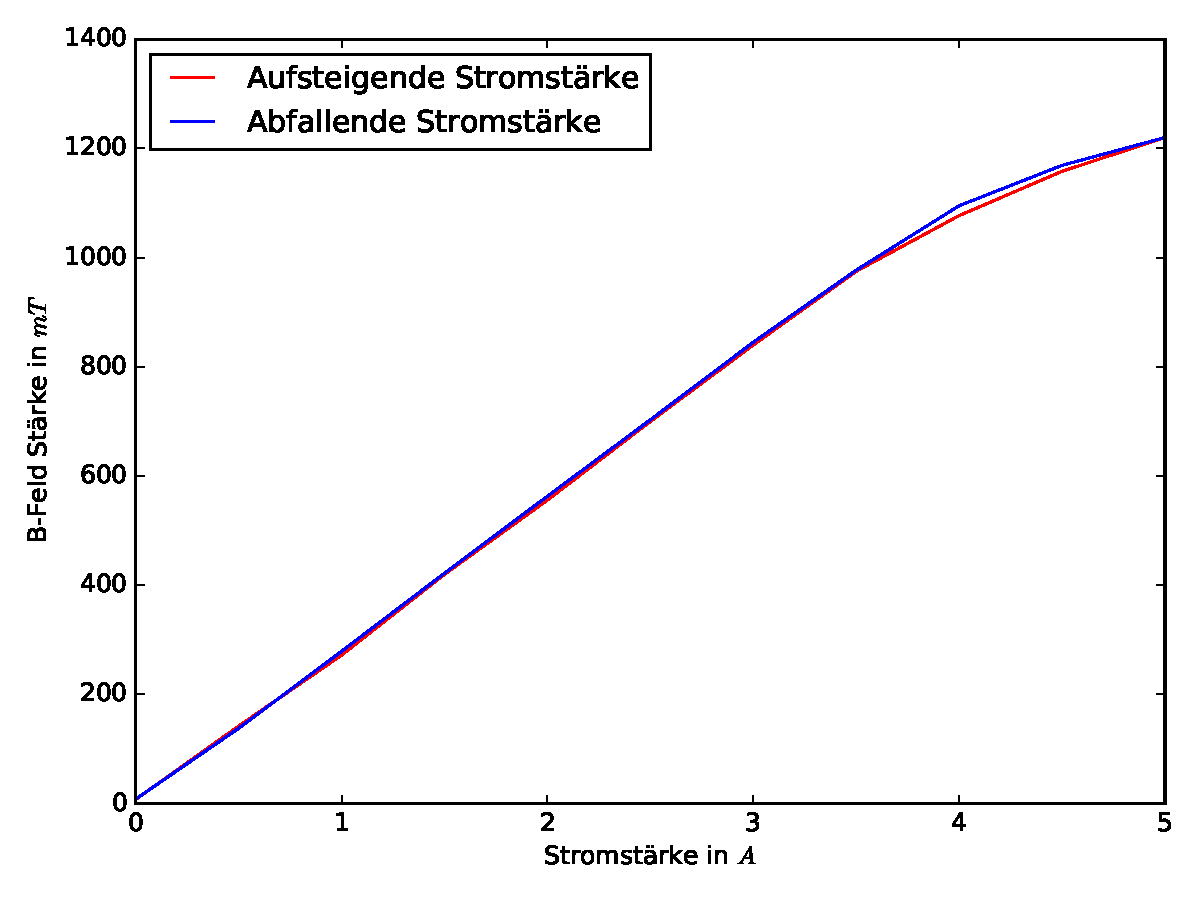
\includegraphics[width=\textwidth]{Hysterese.pdf}
  \caption{Der auftretende Hystereseeffekt: B-Feldstärke aufgetragen gegen die Stromstärke}
  \label{fig:Hysterese}
\end{figure}

In dem Diagramm wird deutlich, dass sich die Verläufe der $B$-Feldstärke bei
unterschiedlich geregelter Stromstärke kaum unterscheiden. Daran ist ersichtlich,
dass der Hystereseeffekt bei der Auswertung der Messergebnisse nur einen vernachlässigbaren
Einfluss besitzt.

Bei den im Versuch angestellten Messungen wurde stets die Stromstärke hochgeregelt,
sodass die $B$-Feldstärke gegenüber des aufgedrehten Stroms verwendet wird, um
den Proportionalitätsfaktor zwischen der Stromstärke $I$ und $B$ zu ermitteln.
Der lineare Fit ist in dem folgendem Diagramm dargestellt.

\begin{figure}
  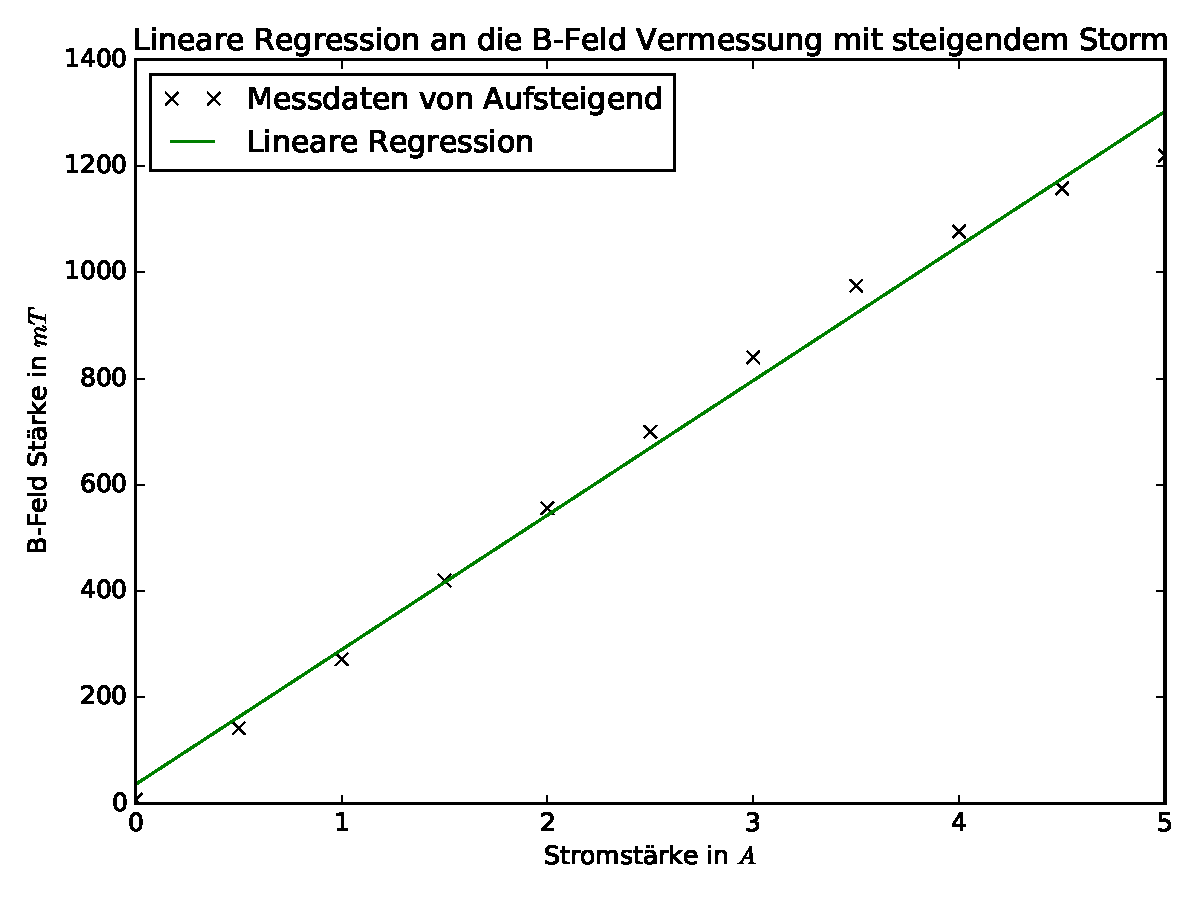
\includegraphics[width=\textwidth]{lineareRegression.pdf}
  \caption{'Lineare Regression an die $B$-Feldstärke bei aufsteigendem $I$'}
  \label{fig:lineareRegression}
\end{figure}

Als Proportionalitätsfaktor zwischen $I$ und $B$ ergibt sich somit $B =
253,35 * I$. Der Proportionalitätsfaktor wird als fehlerfrei angenommen.

\subsection{Messung der Widerstände}

Die Widerstände lassen sich über die Messergebnisse der Spannung bei variierender
Stromstärke errechnen. Das Ohmsche Gesetz besagt, dass der Widerstand der
Proportionalitätsfaktor zwischen der Spannung und der Stromstärke ist.
In den folgenden Diagrammen ist die Spannung gegenüber der Stromstärke aufgetragen.
Die Regressionsgerade wurde direkt in Diagramme integriert.

\begin{figure}
  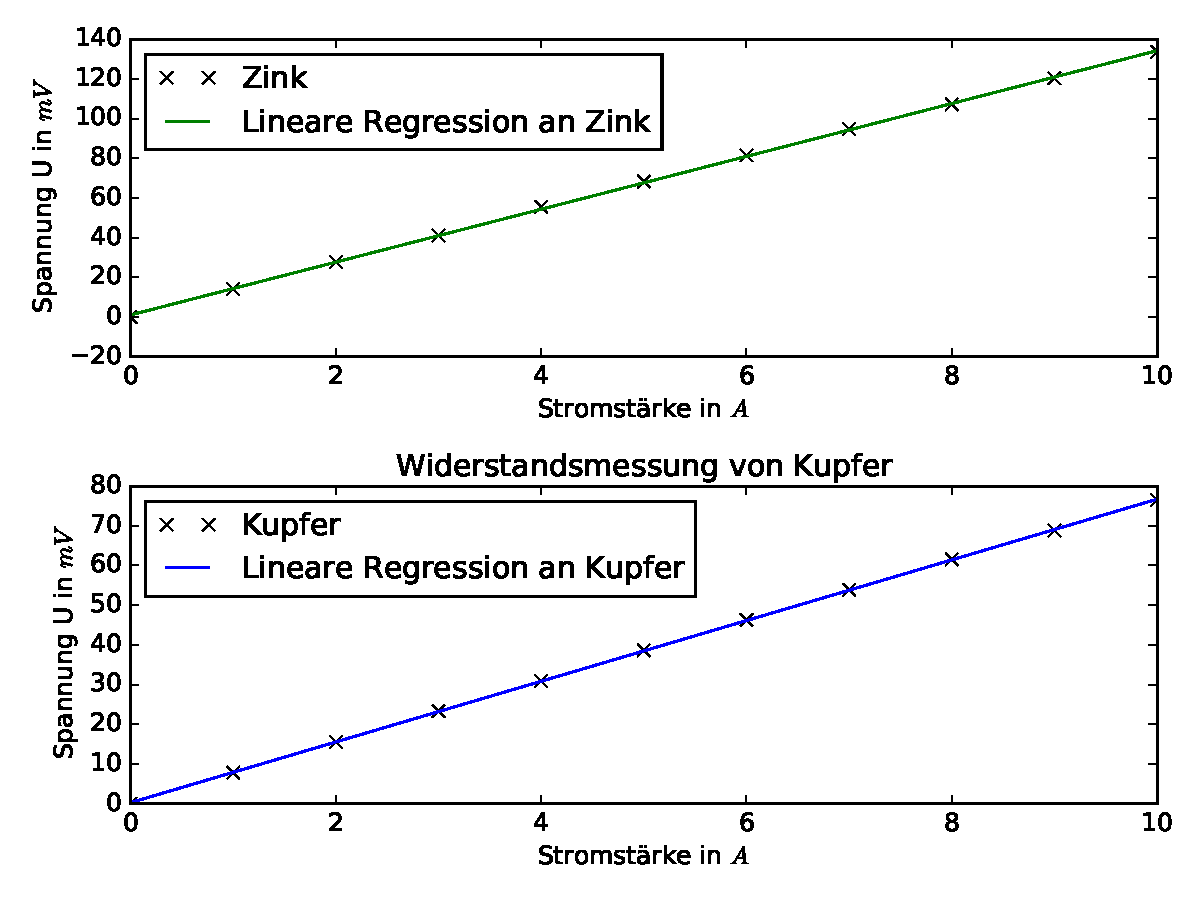
\includegraphics[width=\textwidth]{Widerstandsmessung.pdf}
  \caption{Diagramme der Widerstandsmessung}
  \label{fig:Widerstände}
\end{figure}

Es ergibt sich für die Zinkprobe ein gemessener Widerstand von $R_Z =
\SI{13,32\pm0,067}{\milli\ohm}$. Für die Kupferprobe ergibt sich ein gemesserner
Widerstand von $R_K = \SI{7,64\pm0,016}{\milli\ohm}$.

\subsection{Bestimmen der Hall--Spannung $U_H$}

Die Hall--Spannung wurde nun unter variierenden Bedingungen gemessen.
Bei der ersten Messung wurde der Probenstrom konstant gelassen und der
Spulenstrom aufgedreht, wodurch die $B$-Feldstärke erhöht wird. Bei der zweiten
Messung wurde die vorgehensweise umgekehrt. Der Spulenstrom wurde konstant gelassen
und der Probenstrom wurde aufgedreht.
Die Messdaten der ersten Messung sind aus den Tabellen \ref{tab:Zink_U_H},
\ref{tab:Kupfer_U_H}, \ref{tab:Zink_U_H_umgepolt} und \ref{tab:Kupfer_U_H_umgepolt}
zu entnehmen.
Die Messdaten der zweiten Messung sind in den Tabellen \ref{tab:Zink_U_H_2},
\ref{tab:Kupfer_U_H_2}, \ref{tab:Zink_U_H_2_umgepolt} und \ref{tab:Kupfer_U_H_2_umgepolt}
dargestellt.
Die folgenden Diagramme visualisieren die gemessenen Daten.

\begin{figure}
  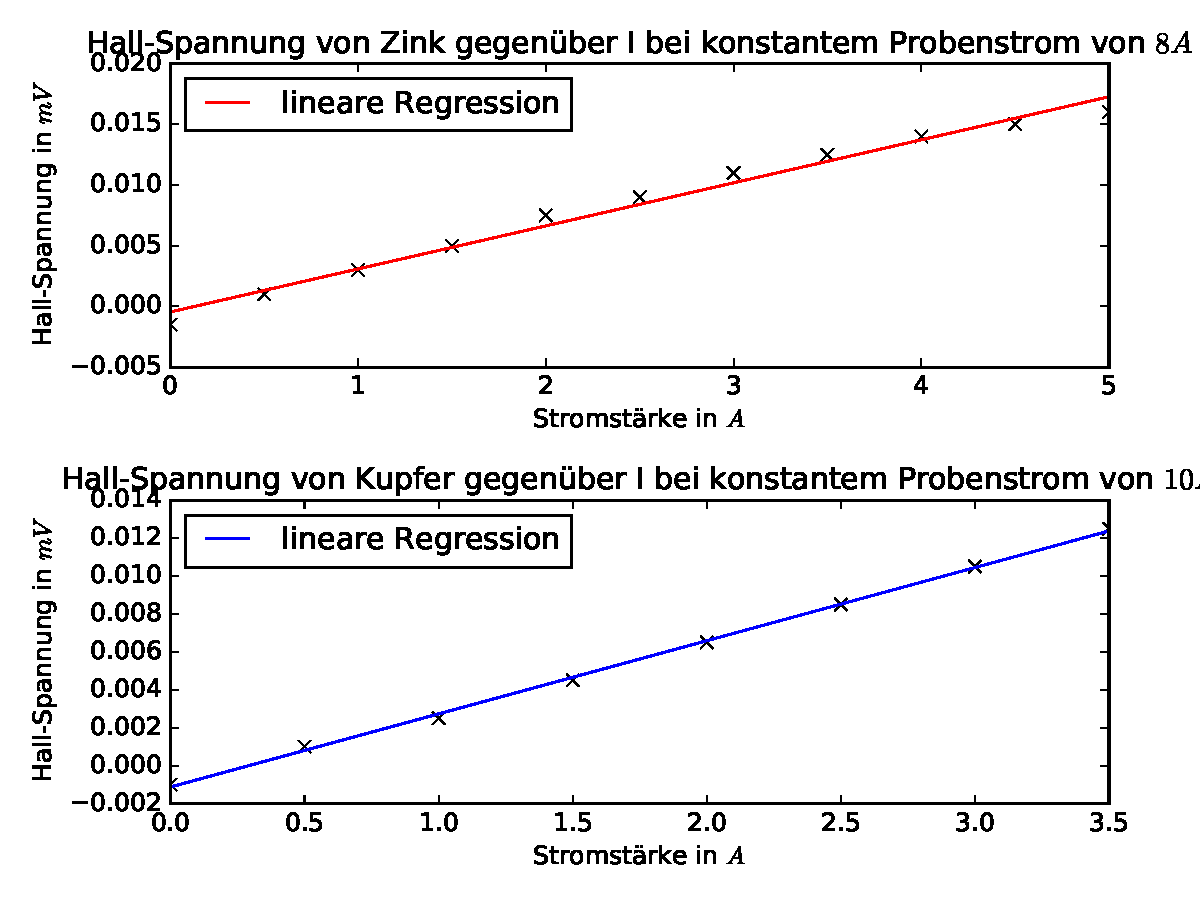
\includegraphics[width=\textwidth]{Hall_Spannung_gegenueber_I_s.pdf}
  \label{fig:U_H_const_Ip}
\end{figure}

\begin{figure}
  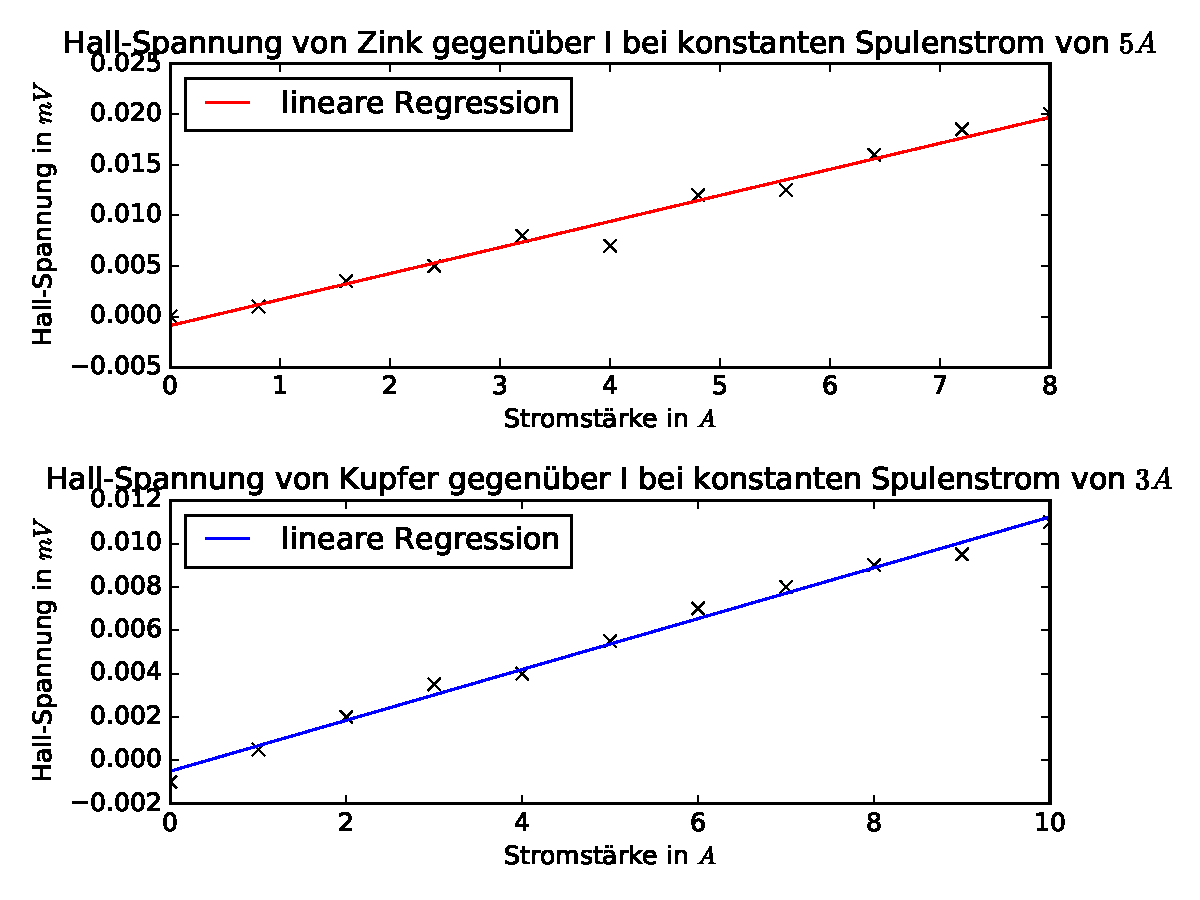
\includegraphics[width=\textwidth]{Hall_Spannung_gegenueber_I_p.pdf}
  \label{fig:U_H_const_Is}
\end{figure}
\FloatBarrier

Die zu den Regressionsgeraden aus den letzten beiden Diagrammen sind
durch \eqref{eqn:Steigung_Zink_I_p} und \eqref{eqn:Steigung_Kupfer_I_p}
gegeben.

\begin{align}
  \label{eqn:Steigung_Zink_I_p}
  m_{1, Zink} &= (\num{1,40 \pm 0,06})\cdot 10^{-5}\si{\volt\per\tesla}\\
  \label{eqn:Steigung_Kupfer_I_p}
  m_{1, Kupfer} &= (\num{-1,52 \pm 0,02})\cdot 10^{-5}\si{\volt\per\tesla}
\end{align}

Über den zuvor bestimmten Proportionalitätsfaktor kann die Hall-Spannung
der $B$-Feldstärke gegenüber aufgetragen werden. Es ergeben sich damit die
folgenden Diagramme.

\begin{figure}
  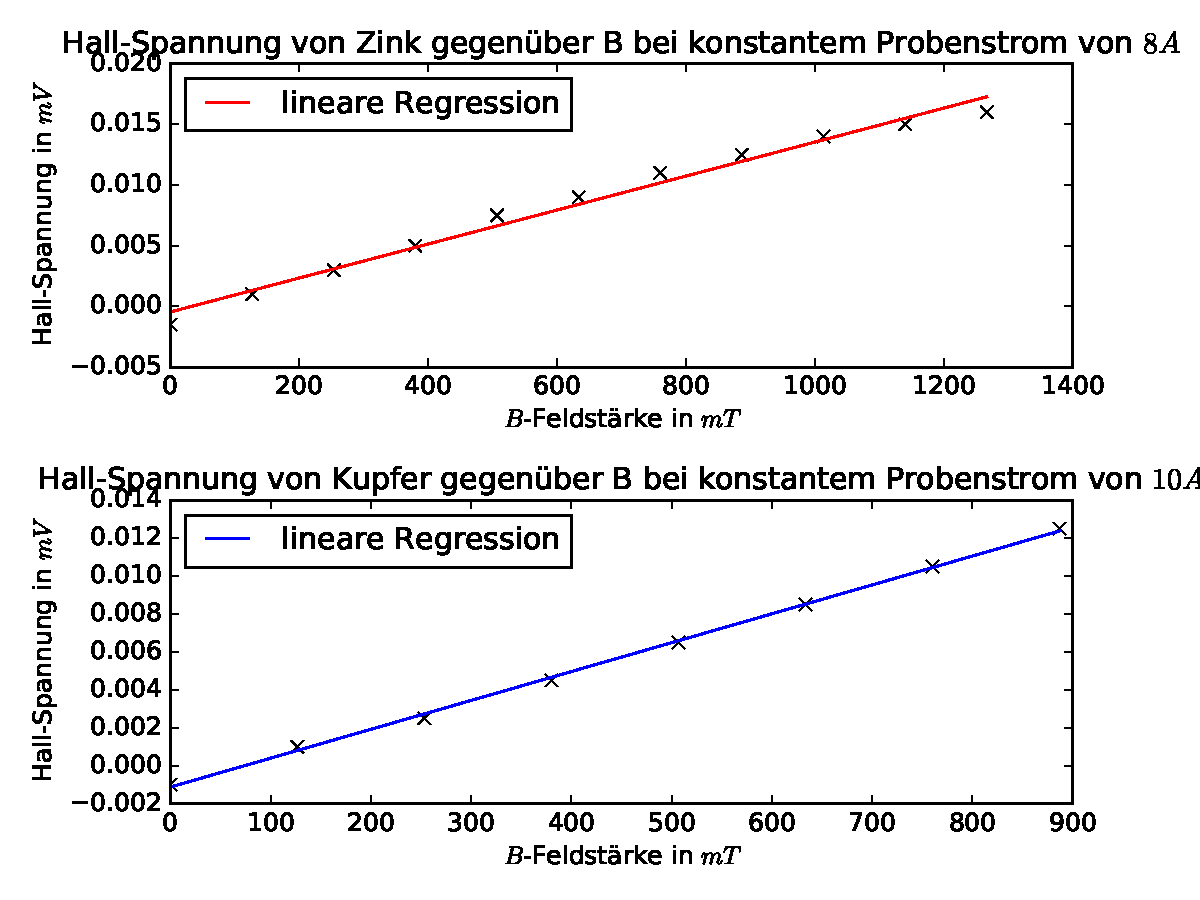
\includegraphics[width=\textwidth]{Hall_Spannung_gegenueber_B_s.pdf}
  \label{fig:U_H_const_Ip_B}
\end{figure}

Die zugehörigen Steigungen der Regressionsgraden sind im Folgendem dargestellt.

\begin{align}
  \label{eqn:Steigung_Zink_Ip_B}
  m_{2, Zink} &= (\num{-2,57 \pm 0,12})\cdot 10^{-3}\si{\volt\per\tesla}\\
  \label{eqn:Steigung_Kupfer_Ip_B}
  m_{2, Kupfer} &= (\num{1,17 \pm 0,04})\cdot 10^{-3}\si{\volt\per\tesla}
\end{align}

Mit Hilfe der Steigungen \eqref{eqn:Steigung_Zink_I_p}, \eqref{eqn:Steigung_Kupfer_I_p},
\eqref{eqn:Steigung_Zink_Ip_B} und \eqref{eqn:Steigung_Kupfer_Ip_B}
lässt sich die Ladungsträgerdichte pro Volumen berechnen.

\subsection{Bestimmen mikroskopischer Leitfähigkeitsparamter}

In diesem Abschnitt werden mit Hilfe der Messergebnisse für die Hall-Spannung und die
Widerstände der Proben mikroskopische Leitfähigkeitsparameter bestimmt.
Zuerst wurde die Ladungsträgeranzahl pro Volumen ermittelt.
Diese ergibt sich aus umstellen der Formel \eqref{eqn:Hall_Spannung} nach $n$ zu:

\begin{equation}
  n = -\frac{B\cdot I_q}{e_0 U_H d}.
\end{equation}

Für die Messungen bei konstantem Probenstrom ergeben sich die Werte

\begin{align*}
  n_{Zink} &= (\num{8,30\pm 0,34})\cdot 10^{27}\frac{1}{\si{\meter^3}}\\
  n_{Kupfer} &= (\num{2,278\pm 0,30})\cdot 10^{29}\frac{1}{\si{\meter^3}}.
\end{align*}

Für die Messungen bei konstantem Spulenstrom ergeben sich die Werte

\begin{align*}
  n_{{Zink}} &= (\num{7,14\pm 0,34}) \cdot 10^{27}\frac{1}{\si{\meter^3}}\\
  n_{{Kupfer}} &= (\num{2,25\pm 0,07})\cdot10^{29}\frac{1}{\si{\meter^3}}.
\end{align*}

Die Zahl der Ladungsträger pro Atom $z$ lässt sich über die folgende Formel bestimmen

\begin{equation}
  z = n \cdot V
\end{equation}
,wobei $n$ die Ladungsträgerdichte pro Volumen ist und $V$ das Molarevolumen ist.

Es ergeben sich für die Zahl der Ladungsträger pro Atom bei konstantem
Querstrom die folgenden Werte

\begin{align*}
  z_{Zink} &= \SI{0,0502\pm0,0021}{\mol\per\meter^3}\\
  z_{Kupfer} &= \SI{2,680\pm0,35}{\mol\per\meter^3}.
\end{align*}

Bei konstentem Spulenstrom ergeben sich

\begin{align*}
  z_{Zink} &= \SI{0,0432\pm0,0021}{\mol\per\meter^3}\\
  z_{Kupfer} &= \SI{2,64\pm0,08}{\mol\per\meter^3}.
\end{align*}

Nach Bestimmen der Ladungsträgerdichte kann die mittlere Flugzeit $\bar{\tau}$
über die Formel \eqref{eqn:mittlereZeit} ermittelt werden.
Aus den Messungen ergeben sich die folgenden Werte. Für die Ladungsträgerdichte
bei konstantem Querstrom ergeben sich

\begin{align*}
\bar{\tau}_{Zink} &= (\num{2,53\pm 0,10})\cdot 10^{-13}\si{\second}\\
\bar{\tau}_{Kupfer} &= (\num{2,046\pm 0.027})\cdot 10^{-13}\si{\second}.
\end{align*}

Für die Ladungsträgerdichte bei konstantem Spulenstrom ergeben sich

\begin{align*}
\bar{\tau}_{Zink} &= (\num{2,94\pm 0,14})\cdot 10^{-13}\si{\second}\\
\bar{\tau}_{Kupfer} &= (\num{2,07\pm 0,06})\cdot 10^{-13}\si{\second}.
\end{align*}

Die Driftgeschwindigkeit lässt sich durch den folgenden Zusammenhang
berechen.
\begin{equation}
  v_d = - \frac{j}{n \cdot e_0}
\end{equation}
Dabei ist $j$ die Stromdichte und $n$ die Ladungsträgerdichte pro Volumen.
Für die Driftgeschwindigkeit bei konstatem Querstrom ergeben sich

\begin{align*}
  v_{d,Zink} &= (\num{7,52\pm0,31})\cdot 10^{-4}\si{\meter\per\second}\\
  v_{d,Kupfer} &= (\num{2,74\pm0,04})\cdot 10^{-5}\si{\meter\per\second}.
\end{align*}

Für die Driftgeschwindigkeit bei konstantem Spulenstrom ergeben sich

\begin{align*}
  v_{d,Zink} &= (\num{8,7\pm0,4})\cdot 10^{-4}\si{\meter\per\second}\\
  v_{d,Kupfer} &= (\num{2,78\pm0,08})\cdot 10^{-5}\si{\meter\per\second}.
\end{align*}

Damit die Totalegeschwindigkeit $|\bar{v}|$ und die mittlere freie Weglänge
$\bar{l}$ ermittelt werden kann muss die
Fermie-Energie der Proben bestimmt werden. Es gelten die folgenden Beziehungen.

\begin{align}
  \label{eqn:Fermi_E}
  E_F &= \frac{h^2}{2m_0}\sqrt[3]{\left(\frac{3}{8\pi}n\right)^2}\\
  \label{eqn:Totalgesch}
  |\bar{v}| &\approx \sqrt{\frac{2E_F}{m_0}}\\
  \label{eqn:l}
  \bar{l} &\approx \bar{\tau}\sqrt{\frac{2E_F}{m_0}}.
\end{align}

Somit lässt sich die Totalgeschwindigkeit allein durch das Bestimmen von $n$
approximieren.

Aus den Messdaten ergeben sich für bei konstantem Querstrom

\begin{align*}
  E_{F,Zink} &= (\num{2,39\pm0,07}) \si{\eV}\\
  E_{F,Kupfer} &= (\num{0,218\pm0,002})\si{\eV}.
\end{align*}

Für die Messungen mit konstantem Spulenstrom ergibt sich

\begin{align*}
  E_{F,Zink} &= (\num{2,17\pm0,07}) \si{\eV}\\
  E_{F,Kupfer} &= (\num{0,216\pm0,004})\si{\eV}.
\end{align*}

Nun kann über die Formel \eqref{eqn:Totalgesch} die Totalgeschwindigkeit errechnet werden. Die folgenden Werte sind bei konstantem Querstrom.

\begin{align*}
  |\bar{v}|_{Zink} &= (1,555\pm 0,021) \cdot 10^{6} \si{\meter\per\second}\\
  |\bar{v}|_{Kupfer} &= (4,692\pm0,020) \cdot 10^6 \si{\meter\per\second}
\end{align*}

Für die Messungen bei konstantem Spulenstrom ergeben sich die folgenden Werte.

\begin{align*}
  |\bar{v}|_{Zink} &= (1,48\pm 0,023) \cdot 10^{6} \si{\meter\per\second}\\
  |\bar{v}|_{Kupfer} &= (4,67\pm0,05) \cdot 10^6 \si{\meter\per\second}
\end{align*}

Desweiteren kann die mittlere freie Weglänge über \eqref{eqn:l} bestimmt werden.
Für die Messdaten bei konstantem Querstrom ergenen sich

\begin{align*}
  \bar{l}_{Zink} &= (\num{0,393\pm0,011})\si{\micro\meter}\\
  \bar{l}_{Kupfer} &= (\num{0,960\pm0,009})\si{\micro\meter}.
\end{align*}

Anhand der Messdaten bei kostantem Spulenstrom ergeben sich die folgenden Werte.

\begin{align*}
  \bar{l}_{Zink} &= (\num{0,435\pm0,014})\si{\micro\meter}\\
  \bar{l}_{Kupfer} &= (\num{0,969\pm0,020})\si{\micro\meter}
\end{align*}

Zwischen $\bar{\tau}$ und der Beweglichkeit $\mu$ besteht der folgende Zusammenhang.

\begin{equation}
  \label{eqn:mu}
  \mu = \frac{e_0}{2m_0}\bar{\tau}
\end{equation}

Darüber ergeben sich bei konstantem Probenstrom die beiliegenden Werte.

\begin{align*}
  \mu_{Zink} &= (\num{0,0222\pm0,0009})\si{\ampere\second^2\per\kilo\gram}\\
  \mu_{Kupfer} &= (\num{0,0180\pm0,00024})\si{\ampere\second^2\per\kilo\gram}
\end{align*}

Bei konstantem Spulenstrom entstehen die Widerstandsmessung
\begin{align*}
  \mu_{Zink} &= (\num{0,0258\pm0,0012})\si{\ampere\second^2\per\kilo\gram}\\
  \mu_{Kupfer} &= (\num{0,0182\pm0,0006})\si{\ampere\second^2\per\kilo\gram}.
\end{align*}

\section{Diskussion}

Abschließend werden die Ergebnisse der Auswertung diskutiert und hingehend ihrer
Aussagekraft bewertet. Zunächst werden mögliche Messungenauigkeiten erläutert.
Die Maße der Proben wurde mittels einer Schieblehre gemessen. Die Proben wiesen
dahingehend Mängel auf, dass ihre Maße nur ungenau bestimmt werden konnten, da sie
durch vorherige Messungen anderer Gruppen schon deformiert waren. Zudem konnte
die Dicke der Proben nur schwierig gemessen werden, da die Proben fixiert waren.
In der Auswertung wurden die Maße als fehlerfrei angenommen, weshalb die Aussagekraft
der ermittelten Größen eingeschränkt wird. Darüberhinaus machte das Voltmeter keinen
zuverlässigen Eindruck, weil es häufig zwischen willkürlich scheinenden Werten
herschwankte. Es musste ein Moment abgepasst werden, bei dem das Voltmeter zuverlässig
schien. Die Messungen konnten aus diesem Grund auch nicht widerholt werden, ohne
völlig verschiedene Resultate zu erhalten. Die Magnetfeldstärke wurde mit Hilfe
einer Hall-Sonde bestimmt und ebenfalls als fehlerfrei angenommen.
Dadurch wird die Aussagekraft der erhaltenen Ergebnisse weiter beschnitten.
Anhand der aufgeführten Argumente wird deutlich, dass die Ergebnisse deutlich
durch Messfehler in ihrer Aussagekraft beschränkt sind. Bei der Messung
des Hystereseeffektes wird deutlich, dass dieser zu vernachlässigen ist.

Bei der Messung für die Kupferprobe traten erhebliche Schwierigkeiten auf, so dass
die Messung abgebrochen und mithilfe des anderen Versuchpaares eine zweite
Kupferprobe ausgewertet wurde. Für diese Probe wurden dann sowohl die Abmessungen
als auch die Messung der Spannungen bei verschiedenen Stromstärken wiederholt.

Ausgehend von der Tatsache, dass Kupfer ein Elektronenleiter ist, ist die
Probe Zink als Löcherleiter zu bewerten.


\end{document}
